\documentclass[cal1spr16Lectures.tex]{subfiles}

\begin{document}

\section[Week 1]{Week 1: 26-29 May}

% % %
%\subsubsection{Tuesday 26 May}
%\begin{frame}{Tues 26 May (Week 1)}
%\begin{itemize}
%\item Syllabus: go to 
%{\footnotesize\url{comp.uark.edu/~ashleykw/Cal1Sum2015/cal1sum15.html}}
%\item All MLP homework for the term is live, but there are due dates.
%\item {\bf 1st MLP hw due...}
%\item For old Calculus materials, see \url{comp.uark.edu/~ashleykw} and look for links under ``Previous Semesters".  Last semester's in-class exam solutions are posted in there, too.
%\end{itemize}
%\end{frame}

% % %
\subsubsection{Tips for Success}
\begin{frame}{Tips for Success}\footnotesize
\begin{itemize}
\item Attend class every day.  \alert{Participate}, take notes, and ask questions.
\item Don't get behind on MLP homeworks.  Stay on top of the book problems.
\item Be sure to seek assistance (tutoring, office hours, etc.) if you are struggling.
\item Don't rely on success in high school calculus to save you in college calculus.
\item Find a study partner(s) to meet with on a regular basis to cover questions and study for quizzes/exams.
\item REMEMBER... THE TERM STARTS TODAY!  SO DOES THE EVENTUAL EARNING OF YOUR FINAL GRADE!!!
\end{itemize}
\end{frame}

% % %
\subsection[2.1 The Idea of Limits]{$\S$2.1 The Idea of Limits}
% % %

% % % 
\begin{frame}{\S 2.1 The Idea of Limits}
\begin{que} How would you define, and then differentiate between, the following pairs of terms? 
\begin{itemize}
\item instantaneous velocity vs. average velocity?
\item tangent line vs. secant line? 
\end{itemize}
\end{que}

(Recall: What is a tangent line and what is a secant line?)
\end{frame}

% % %
\begin{frame}\footnotesize
\begin{ex} An object is launched into the air. Its position $s$ (in feet) at any time $t$ (in seconds) is given by the equation:
\[s(t)=-4.9t^2+30t+20.\]
\hrulefill
\begin{itemize}
\item[(a)] Compute the average velocity of the object over the following time intervals:  $[1,3],\,[1,2],\,[1,1.5]$
\item[(b)] As your interval gets shorter, what do you notice about the average velocities?  What do you think would happen if we computed the average velocity of the object over the interval $[1,1.2]$? $[1,1.1]$? $[1,1.05]$?
\end{itemize}
\end{ex}
\end{frame}

% % %
\begin{frame}\footnotesize
\begin{block}{Example, cont.} An object is launched into the air. Its position $s$ (in feet) at any time $t$ (in seconds) is given by the equation:
\[s(t)=-4.9t^2+30t+20.\]
\hrulefill
\begin{itemize}
\item[(c)] How could you use the average velocities to estimate the instantaneous velocity at $t=1$?
\item[(d)] What do the average velocities you computed in 1.\ represent on the graph of $s(t)$?
\end{itemize}
\end{block}
\end{frame}

% % %
\begin{frame}
\begin{que} What happens to the relationship between \alert{instantaneous} velocity and \alert{average} velocity as the time interval gets shorter? \end{que}

{\bf Answer:} The instantaneous velocity at $t=1$ is the limit of the average velocities as $t$ approaches 1.
\end{frame}

% % %
\begin{frame}
\begin{que} What about the relationship between the \alert{secant} lines and the \alert{tangent} lines as the time interval gets shorter? \end{que}

{\bf Answer:} The slope of the tangent line at $(1, 45.1=s(1))$ is the limit of the slopes of the secant lines as $t$ approaches 1.
\end{frame}

% % %
\subsubsection{Book Problems}
\begin{frame}
\begin{block}{2.1 Book Problems}1-3, 7-13, 15, 21, 25, 27, 29\end{block}
%\begin{itemize}
%\item 
Even though book problems aren't turned in, they're a very good way to study for quizzes and tests (wink wink wink).  
%\end{itemize}
\end{frame}

% % %
\subsection[2.2 Definition of Limits]{\S 2.2 Definition of Limits}
% % %

% % %
\begin{frame}{\S 2.2 Definition of Limits}
\begin{que} 
\begin{itemize}
	\item Based on your everyday experiences, how would you define a ``limit"? 
	\item Based on your mathematical experiences, how would you define a ``limit"?
	\item How do your definitions above compare or differ?
\end{itemize}
\end{que}
\end{frame}

% % % 
\subsubsection{Definition of a Limit of a Function}
\begin{frame}{\small Definition of a Limit of a Function}
\begin{dfn}[limit]
Suppose the function $f$ is defined for all $x$ near $a$, except possibly at $a$.  If $f(x)$ is arbitrarily close to $L$ (as close to $L$ as we like) for all $x$ sufficiently close (but not equal) to $a$, we write
\[
\lim_{x\to a}f(x)=L
\]
and say \textbf{the limit of $f(x)$ as $x$ approaches $a$ equals $L$}.
\end{dfn}
\end{frame}

% % %
\subsubsection{Determining Limits from a Graph}
\begin{frame}{\small Determining Limits from a Graph}
\begin{exe}
\begin{columns}
\begin{column}{0.45\textwidth}
	\centering{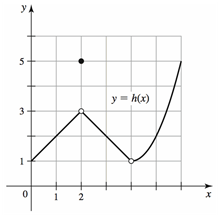
\includegraphics[scale=0.85]{pictures/Ch2Sect2_Exer7}}
\end{column}
\begin{column}{0.50\textwidth}\footnotesize
	Determine the following:

	\vspace{-0.4pc}
	\begin{itemize}\footnotesize
	\item[(a)] $h(1)$
	
	\vspace{-0.25pc}
	\item[(b)] $h(2)$
	
	\vspace{-0.25pc}
	\item[(c)] $h(4)$
	
	\vspace{-0.25pc}
	\item[(d)] $\lim_{x \to 2} h(x)$
	
	
	\vspace{-0.25pc}
	\item[(e)] $\lim_{x \to 4} h(x)$
	
	\vspace{-0.25pc}
	\item[(f)] $\lim_{x \to 1} h(x)$
	\end{itemize}
\end{column}
\end{columns}
\end{exe}
\end{frame}

% % %
\begin{frame}
\begin{que} Does $\lim_{x \to a} f(x)$ always equal $f(a)$? \end{que}
(Hint: Look at the example from the previous slide!)
\end{frame}

% % %
\subsubsection{Determining Limits from a Table}
\begin{frame}{\small Determining Limits from a Table}
\begin{exe} Suppose $f(x)=\dfrac{x^2+x-20}{x-4}$.

\begin{itemize}
\item[(a)] Create a table of values of $f(x)$ when
\begin{alignat*}{3}
x &= 3.9, 3.99, 3.999,\ \text{and}\\
x &= 4.1, 4.01, 4.001
\end{alignat*}
\item[(b)] What can you conjecture about $\lim_{x \to 4} f(x)$?
\end{itemize}
\end{exe}
\end{frame}

% % %
\subsubsection{One-Sided Limits}
\begin{frame}{\small One-Sided Limits}
Up to this point we have been working with two-sided limits; however, for some functions it makes sense to examine one-sided limits.  

\vspace{2pc}
Notice how in the previous example we could approach $f(x)$ from both sides as $x$ approaches $a$, i.e., when $x>a$ and when $x<a$.  
\end{frame} 

% % %
\begin{frame}\footnotesize
\begin{dfn}[right-hand limit] Suppose $f$ is defined for all $x$ near $a$ with $x>a$.  If $f(x)$ is arbitrarily close to $L$ for all $x$ sufficiently close to $a$ with $x>a$, we write

\vspace{-0.5pc}
\[\lim_{x \to a^+} f(x)=L\]

\vspace{-0.25pc}
and say {\bf the limit of $f(x)$ as $x$ approaches $a$ from the right equals $L$}. \end{dfn}

\begin{dfn}[left-hand limit] Suppose $f$ is defined for all $x$ near $a$ with $x<a$.  If $f(x)$ is arbitrarily close to $L$ for all $x$ sufficiently close to $a$ with $x<a$, we write

\vspace{-0.5pc}
\[\lim_{x \to a^-} f(x)=L\]

\vspace{-0.25pc}
and say {\bf the limit of $f(x)$ as $x$ approaches $a$ from the left equals $L$}. \end{dfn}
\end{frame}

% % %
\begin{frame}
\begin{exe}
\begin{columns}
\begin{column}{.45\textwidth}
	\centering{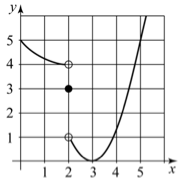
\includegraphics[scale=1]{pictures/Ch2Sect2_QQ7}}
\end{column}
\begin{column}{.45\textwidth}
	Determine the following:
	
	\vspace{0.25pc}
	\begin{itemize}
	\item[(a)] $g(2)$

	\vspace{0.25pc}	
	\item[(b)] $\lim_{x \to 2^+} g(x)$
	
	\vspace{0.25pc}
	\item[(c)] $\lim_{x \to 2^-} g(x)$
	
	\vspace{0.25pc}
	\item[(d)] $\lim_{x \to 2} g(x)$
	\end{itemize}
	\vspace{3pc}
\end{column}
\end{columns}
\end{exe}
\end{frame}

% % %
\subsubsection{Relationship Between One- and Two-Sided Limits}
\begin{frame}{\small Relationship Between One- and Two-Sided Limits}
\begin{thm}\footnotesize If $f$ is defined for all $x$ near $a$ except possibly at $a$, then $\lim_{x \to a} f(x)=L$ if and only if \alert{both} $\lim_{x \to a^+} f(x)=L$ \alert{and} $\lim_{x \to a^-} f(x)=L$. \end{thm}

In other words, the only way for a two-sided limit to exist is if the one-sided limits equal the same number ($L$).
\end{frame}

% % %
\subsubsection{Book Problems}
\begin{frame}
\begin{block}{2.2 Book Problems}1-4, 7, 9, 11, 13, 19, 23, 29, 31 \end{block} 
\end{frame}

% % %
\subsection[2.3 Techniques for Computing Limits]{\S 2.3 Techniques for Computing Limits}
% % %

% % %
\begin{frame}{\S 2.3 Techniques for Computing Limits}\footnotesize
\begin{exe}
Given the function $f(x)=4x+7$, find $\lim_{x\to -2}f(x)$
\begin{enumerate}[(a)]
	\item graphically;
	\item numerically (i.e., using a table of values near $-2$)
	\item via a direct computation method of your choosing.
	\end{enumerate}
\end{exe}

Compare and contrast the methods in this exercise -- which is the most favorable?
\end{frame}

% % %
\begin{frame}{}\footnotesize
This section provides various laws and techniques for determining limits.  These constitute {\bf analytical} methods of finding limits.  The following is an example of a very useful limit law:

\vspace{0.5pc}
{\bf Limits of Linear Functions:}  Let $a$, $b$, and $m$ be real numbers.  For linear functions $f(x)=mx+b$,

\vspace{-0.5pc}
\[\lim_{x \to a} f(x)=f(a)=ma+b.\]

\vspace{0.25pc}
This rule says if $f(x)$ is a linear function, then in taking the limit as $x\to a$, we can just plug in the $a$ for $x$.

\vspace{0.5pc}
\alert{IMPORTANT!} Using a table or a graph to compute limits, as in the previous sections, can be helpful.  However, ``analytical" does not include those techniques.
\end{frame}

% % %
\subsubsection{Limit Laws}
\begin{frame}{\small Limit Laws}{}
{\footnotesize Assume $\lim_{x \to a} f(x)$ and $\lim_{x \to a} g(x)$ exist, $c$ is a real number, and $m,n$ are positive integers.

\hrulefill
}
\begin{itemize}
\item[{\bf 1.}] {\bf Sum:} $\lim_{x \to a}\left(f(x)+g(x)\right) = \lim_{x \to a} f(x)+\lim_{x \to a} g(x)$

\vspace{1pc}
\item[{\bf 2.}] {\bf Difference:} $\lim_{x \to a}\left(f(x)-g(x)\right) = \lim_{x \to a} f(x)-\lim_{x \to a} g(x)$
\end{itemize}

\vspace{1.25pc}In other words, if we are taking a limit of two things added together or subtracted, then we can first compute each of their individual limits one at a time.
\end{frame}

% % %
\begin{frame}{\small Limit Laws, cont.}{}
{\footnotesize Assume $\lim_{x \to a} f(x)$ and $\lim_{x \to a} g(x)$ exist, $c$ is a real number, and $m,n$ are positive integers.

\hrulefill
}
\begin{itemize}
\item[{\bf 3.}] {\bf Constant Multiple:} $\lim_{x \to a}\left(cf(x)\right) = c\left(\lim_{x \to a}f(x)\right)$

\vspace{1pc}
\item[{\bf 4.}] {\bf Product:}  $\lim_{x \to a}\left(f(x)g(x)\right) = \left(\lim_{x \to a} f(x)\right) \left(\lim_{x \to a} g(x)\right)$
\end{itemize}

\vspace{1.25pc}
The same is true for products.  If one of the factors is a constant, we can just bring it outside the limit.  In fact, a constant is its own limit.
\end{frame}

% % %
\begin{frame}{\small Limit Laws, cont.}{}
{\footnotesize Assume $\lim_{x \to a} f(x)$ and $\lim_{x \to a} g(x)$ exist, $c$ is a real number, and $m,n$ are positive integers.

\hrulefill
}
\begin{itemize}
\item[{\bf 5.}] {\bf Quotient:}  $\lim_{x \to a} \left(\frac{f(x)}{g(x)} \right) = \frac{\displaystyle\lim_{x \to a} f(x)}{\displaystyle\lim_{x \to a} g(x)}$

\vspace{1pc}
(provided $\lim_{x \to a} g(x) \ne 0$)
\end{itemize}

\begin{que}Why the caveat? \end{que}
\end{frame}

% % %
\begin{frame}{\small Limit Laws, cont.}{}\footnotesize
{\footnotesize Assume $\lim_{x \to a} f(x)$ and $\lim_{x \to a} g(x)$ exist, $c$ is a real number, and $m,n$ are positive integers.

\hrulefill
}
\begin{itemize}
\item[{\bf 6.}] {\bf Power:} $\lim_{x \to a}\left(f(x)\right)^n = \left( \lim_{x \to a} f(x) \right)^n$

\vspace{0.4pc}
\item[{\bf 7.}] {\bf Fractional Power:} $\lim_{x \to a} \left(f(x)\right)^{\frac{n}{m}} = \left( \lim_{x \to a} f(x) \right)^{\frac{n}{m}}$ 

\vspace{0.2pc}
(provided $f(x) \ge 0$ for $x$ near $a$ if $m$ is even and $\textstyle\frac{n}{m}$ is in lowest terms)
\end{itemize}

\vspace{-0.3pc}
\begin{que}Explain the caveat in {\bf 7.} \end{que}
\end{frame}

% % %
\begin{frame}{\small Limit Laws, cont.}\footnotesize
Laws {\bf 1.}-{\bf 6.} hold for one-sided limits as well.  But {\bf 7.} must be modified:

\begin{itemize}
\item[{\bf 7.}] {\bf Fractional Power (one-sided limits):} 
	\begin{itemize}
	\item $\lim_{x \to a^{\alert{+}}}\left(f(x)\right)^{\frac{n}{m}} = \left( \lim_{x \to a^{\alert{+}}} f(x) \right)^{\frac{n}{m}}$

	\vspace{0.25pc}
	(provided $f(x) \ge 0$ for $x$ near $a$ \alert{with $x>a$}, if $m$ is even and $\textstyle\frac{n}{m}$ is in lowest terms)
	
	\vspace{0.75pc}
	\item $\lim_{x \to a^{\alert{-}}}\left(f(x)\right)^{\frac{n}{m}} = \left( \lim_{x \to a^{\alert{-}}} f(x) \right)^{\frac{n}{m}}$ 
	
	\vspace{0.25pc}
	(provided $f(x) \ge 0$ for $x$ near $a$ \alert{with $x<a$}, if $m$ is even and $\textstyle\frac{n}{m}$ is in lowest terms)
	\end{itemize}
\end{itemize}
\end{frame}

% % %
\subsubsection{Limits of Polynomials and Rational Functions}
\begin{frame}{\small Limits of Polynomials and Rational Functions}{}\footnotesize
Assume that $p(x)$ and $q(x)$ are polynomials and $a$ is a real number.

\vspace{0.6pc}
\begin{itemize}
\item {\bf Polynomials:}  $\lim_{x \to a} p(x) = p(a)$

\vspace{0.4pc}
\item {\bf Rational functions:}  $\lim_{x \to a} \frac{p(x)}{q(x)} = \frac{p(a)}{q(a)}$ 

\vspace{0.1pc}
(provided $q(a) \ne 0$)
\end{itemize}

\vspace{0.6pc} 
For polynomials and rational functions we can plug in $a$ to compute the limit, as long as we don't get zero in the denominator.  Linear functions count as polynomials.  A rational function is a ``fraction" made of polynomials.
\end{frame}

% % %
\begin{frame}\footnotesize
\begin{exe} Evaluate the following limits analytically.
\begin{itemize}
\item[1.\quad] $\lim_{x \to 1}\frac{4f(x)g(x)}{h(x)}$, given that 

\vspace{-0.25pc}
\[\lim_{x \to 1} f(x)=5, \; \lim_{x \to 1} g(x)=-2, \;\text{and }\lim_{x \to 1} h(x)=-4.\]

\vspace{0.1pc}
\item[2.\quad] $\lim_{x \to 3} \frac{4x^2+3x-6}{2x-3}$

\vspace{0.5pc}
\item[3.\quad] $\lim_{x \to 1^-}g(x)$ \;and\; $\lim_{x \to 1^+}g(x)$, given that

\vspace{-0.25pc}
\[g(x) = 
\begin{cases}
x^2 & \text{if $x \le 1$}; \\
x+2 & \text{if $x>1$}.
\end{cases}
\] 
\end{itemize}
\end{exe}
\end{frame}

% % %
\subsubsection{Additional (Algebra) Techniques}
\begin{frame}{\small Additional (Algebra) Techniques}\footnotesize
When direct substitution (a.k.a. plugging in $a$) fails try using algebra:

\vspace{0.25pc}
\begin{itemize}
\item Factor and see if the denominator cancels out.
\begin{ex} $\lim_{t \to 2} \frac{3t^2-7t+2}{2-t}$ \end{ex}

\vspace{0.25pc}
\item Look for a common denominator.
\begin{ex} $\lim_{h \to 0} \frac{ \frac{1}{5+h}-\frac{1}{5} }{h}$ \end{ex}
\end{itemize}
\end{frame}

% % % 
\begin{frame}
\begin{exe}
Evaluate $\lim_{s\to 3}\frac{\sqrt{3s+16}-5}{s-3}$.
\end{exe}
\end{frame}

% % %
\subsubsection{Another Technique: Squeeze Theorem}
\begin{frame}{\small Another Technique: Squeeze Theorem}
This method for evaluating limits uses the relationship of functions with each other.

\begin{thm}[Squeeze Theorem]\footnotesize  Assume $f(x)\leq g(x)\leq h(x)$ for all values of $x$ near $a$, except possibly at $a$, and suppose
\[\lim_{x \to a}f(x)=\lim_{x \to a} h(x)=L.\] 
Then since $g$ is always between $f$ and $h$ for $x$-values close enough to $a$, we must have 
\[\lim_{x \to a} g(x)=L.\] \end{thm}
\end{frame}

% % %
\begin{frame}
\begin{ex} \begin{itemize}
\item[(a)]Draw a graph of the inequality 
\[-|x| \leq x^2 \ln{(x^2)} \leq |x|.\]

\vspace{0.5pc}
\item[(b)] Compute $\lim_{x \to 0} x^2 \ln{(x^2)}.$
\end{itemize}
\end{ex}
\end{frame}

% % %
\subsubsection{Book Problems}
\begin{frame}
\begin{block}{2.3 Book Problems} 12-30 (every 3rd problem), 33, 39-51 (odds), 55, 57, 61-67 (odds) \end{block}
%\begin{itemize}
%\item 
In general, review your algebra techniques, since they can save you some headache.
%\end{itemize}
\end{frame}

\end{document}